\documentclass[12pt, a4paper, oneside]{book}
\usepackage[hidelinks]{hyperref}
\usepackage[slovak]{babel}
\usepackage{epsfig}
\usepackage{epstopdf}
\usepackage[chapter]{algorithm}
\usepackage{algorithmic}
\usepackage{listings}
\usepackage{amsmath}
\usepackage{amssymb}
\usepackage{graphicx}
\usepackage{multirow}
\usepackage{color}
\usepackage{url}
\usepackage[utf8]{inputenc}
\usepackage[T1]{fontenc}
\usepackage{setspace}
\usepackage{tabularx}
\usepackage{textcomp}
\usepackage{caption}
\usepackage{natbib}

\setstretch{1.5}
%\renewcommand\baselinestretch{1.5} % riadkovanie jeden a pol

% pekne pokope definujeme potrebne udaje
\newcommand\mftitle{GPS navigácia peších osôb v meste
	spojená s mestskou hromadnou
	dopravou}
\newcommand\mfthesistype{Diplomová práca}
\newcommand\mfauthor{Bc. Martin Palka}
\newcommand\mfadvisor{RNDr. Marek Nagy, PhD.}
\newcommand\mfplacedate{Bratislava, 2018}
\newcommand\mfuniversity{UNIVERZITA KOMENSKÉHO V BRATISLAVE}
\newcommand\mffaculty{FAKULTA MATEMATIKY, FYZIKY A INFORMATIKY}
\newcommand{\sub}[1]{$_{\text{#1}}$}
\newcommand{\reference}[1]{č.~\ref{#1}}
\newcommand{\imageHeight}{150px}

\ifx\pdfoutput\undefined\relax\else\pdfinfo{ /Title (\mftitle) /Author (\mfauthor) /Creator (PDFLaTeX) } \fi

\begin{document}

\frontmatter

\thispagestyle{empty}

\noindent
\begin{minipage}{\textwidth}
\begin{center}
\textbf{\mfuniversity \\
\mffaculty}
\end{center}
\end{minipage}

\vfill
\begin{figure}[!hbt]
	\begin{center}
		
\includegraphics{images/logo_fmph}
		\label{img:logo}
	\end{center}
\end{figure}
\begin{center}
	\begin{minipage}{0.8\textwidth}
		\centerline{\textbf{\Large\MakeUppercase{\mftitle}}}
		\smallskip
		\centerline{\mfthesistype}
	\end{minipage}
\end{center}
\vfill
2017 \hfill
\mfauthor
\eject 
% koniec obalu

\thispagestyle{empty}

\noindent
\begin{minipage}{\textwidth}
\begin{center}
\textbf{\mfuniversity \\
\mffaculty}
\end{center}
\end{minipage}

\vfill
\begin{figure}[!hbt]
\begin{center}

\includegraphics{images/logo_fmph_dark}
\label{img:logo_dark}
\end{center}
\end{figure}
\begin{center}
\begin{minipage}{0.8\textwidth}
\centerline{\textbf{\Large\MakeUppercase{\mftitle}}}
\smallskip
\centerline{\mfthesistype}
\end{minipage}
\end{center}
\vfill
\begin{tabular}{l l}
%Registration number: & 40a99bd8-3cb6-4534-9330-c7fd9b5e5ca4 \\
Študijný program: & Aplikovaná informatika\\
Študijný odbor: & 2511 Aplikovaná informatika\\
Školiace pracovisko: & Katedra aplikovanej informatiky\\
Školiteľ: & \mfadvisor
\end{tabular}
\vfill
\noindent
\mfplacedate \hfill
\mfauthor
\eject 
% koniec titulneho listu

\thispagestyle{empty}
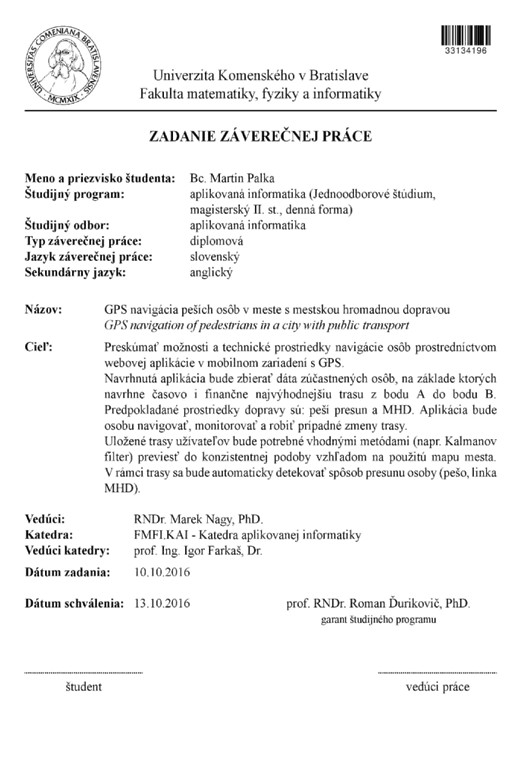
\includegraphics[width=\textwidth]{images/zadaniedp}
\vfill
\eject
% koniec zadania

\thispagestyle{empty}


\begin{figure}[H]
\begin{center}
%\makebox[\textwidth]{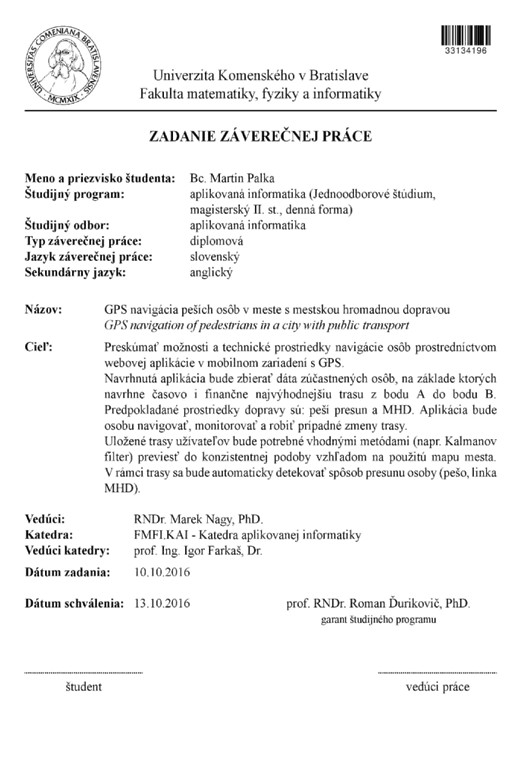
\includegraphics[width=\paperwidth]{images/zadaniedp}}
%\label{img:zadanie}
\end{center}
\end{figure}

{~}\vspace{12cm}

\noindent
\begin{minipage}{0.25\textwidth}~\end{minipage}
\begin{minipage}{0.75\textwidth}
Čestne prehlasujem, že túto diplomovú prácu som vypracoval samostatne len
s použitím uvedenej literatúry a za pomoci konzultácií u môjho školiteľa
\newline \newline
\end{minipage}
\vfill
~ \hfill {\hbox to 6cm{\dotfill}} \\
\mfplacedate \hfill \mfauthor
\vfill\eject 
% koniec prehlasenia

\chapter*{Poďakovanie}\label{chap:thank_you}
Touto cestou by som sa chcel v prvom rade poďakovať môjmu školiteľovi
RNDr. Marekovi Nagymu, PhD. za jeho cenné rady a usmernenia, ktoré mi veľmi pomohli pri
riešení tejto diplomovej práce. Takisto sa chcem poďakovať´ všetkým mojím kamarátom a
celej mojej rodine za podporu počas môjho štúdia
\vfill\eject 
% koniec podakovania

\chapter*{Abstrakt}\label{chap:abstract_sk}
Tato práca sa venuje problematike GPS a navigovania peších po meste spojenej
s mestskou hromadnou dopravou. Súčasnou tejto práce je prehľad existujúcich riešení a ich
krátke zhodnotenie. V práci je popísaný návrh a implementácia nášho modelu, ďalej je tu
popísaná detekcia presunu osôb.
\vfill\eject 

\chapter*{Abstract}\label{chap:abstract_en}
This work deals with the issue of GPS and pedestrian navigation in the city cowith the
city public transport. Part of this work is an overview of existing solutions and their brief
assessment. The thesis olso describes the design and implementation of our model, and there
is described the transfer of persons.
\vfill\eject 
% koniec abstraktov

\tableofcontents

\mainmatter

\input 01intro.tex
\input 02motivation.tex
\input 03issues_overview.tex

\backmatter

\nocite{*}
\bibliographystyle{alpha}
\bibliography{ref}

%\listoffigures

\end{document}